\documentclass{standalone}
\usepackage{tikz}

\begin{document}
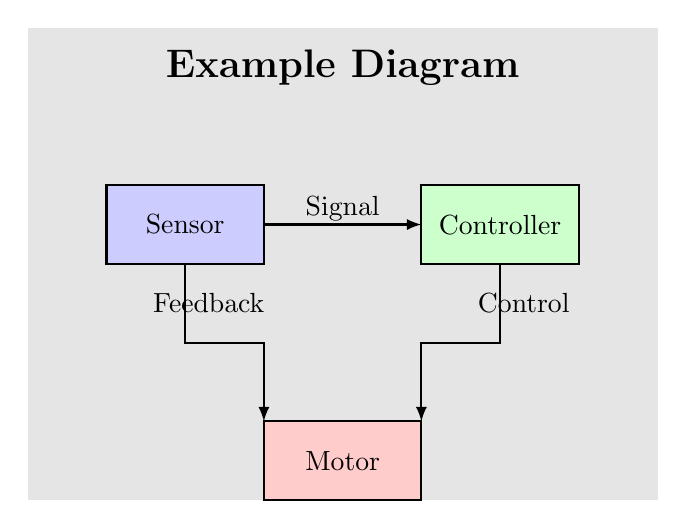
\begin{tikzpicture}
  % Background
  \fill[gray!20] (0,0) rectangle (8,6);
  
  % Title
  \node[font=\bfseries\Large] at (4,5.5) {Example Diagram};
  
  % Boxes
  \draw[fill=blue!20,thick] (1,4) rectangle (3,3) node[midway] {Sensor};
  \draw[fill=green!20,thick] (5,4) rectangle (7,3) node[midway] {Controller};
  \draw[fill=red!20,thick] (3,1) rectangle (5,0) node[midway] {Motor};
  
  % Arrows
  \draw[-latex,thick] (3,3.5) -- (5,3.5);
  \draw[-latex,thick] (6,3) -- (6,2) -- (5,2) -- (5,1);
  \draw[-latex,thick] (2,3) -- (2,2) -- (3,2) -- (3,1);
  
  % Labels
  \node[text width=2cm,align=center] at (4,3.7) {Signal};
  \node[text width=2cm,align=center] at (6.3,2.5) {Control};
  \node[text width=2cm,align=center] at (2.3,2.5) {Feedback};
  
\end{tikzpicture}
\end{document}